% ============================================================
% 讲义 — 人教版高中选择性必修第一册 · 第2章 直线和圆的方程
% 编译命令：xelatex -interaction=nonstopmode 高二选必1_第2章_直线和圆的方程.tex
% ============================================================
\documentclass[12pt, a4paper]{ctexart}
\usepackage[margin=2.2cm]{geometry}
\usepackage{amsmath, amssymb}
\usepackage{enumitem}
\usepackage{tcolorbox}
\usepackage{booktabs}
\usepackage{array}
\usepackage{fancyhdr}
\usepackage{xcolor}
\usepackage{tikz}
\usepackage{hyperref}
\usepackage{graphicx}
\usepackage{multirow}
\usepackage{pgfplots}
\pgfplotsset{compat=1.18}

% 颜色定义
\definecolor{mainblue}{RGB}{41, 98, 168}
\definecolor{lightblue}{RGB}{230, 240, 255}
\definecolor{tipgreen}{RGB}{34, 139, 87}
\definecolor{lightgreen}{RGB}{235, 250, 240}
\definecolor{warnred}{RGB}{200, 50, 50}
\definecolor{lightred}{RGB}{255, 240, 240}
\definecolor{examorange}{RGB}{210, 120, 20}
\definecolor{lightorange}{RGB}{255, 248, 235}
\definecolor{apppurple}{RGB}{120, 60, 170}
\definecolor{lightpurple}{RGB}{245, 238, 255}

% 页眉页脚
\pagestyle{fancy}
\fancyhf{}
\fancyhead[L]{\small\textcolor{mainblue}{\textbf{人教版高中选择性必修第一册}}}
\fancyhead[R]{\small\textcolor{mainblue}{第2章 直线和圆的方程}}
\fancyfoot[C]{\small —\ \thepage\ —}
\renewcommand{\headrulewidth}{0.6pt}
\renewcommand{\headrule}{\hbox to\headwidth{\color{mainblue}\leaders\hrule height \headrulewidth\hfill}}
\renewcommand{\footrulewidth}{0pt}

% tcolorbox 样式
\newtcolorbox{knowledgebox}[1][]{%
  colback=lightblue, colframe=mainblue,
  fonttitle=\bfseries\large, title=#1,
  arc=3mm, boxrule=0.8pt,
  left=8pt, right=8pt, top=6pt, bottom=6pt
}

\newtcolorbox{tipbox}[1][]{%
  colback=lightgreen, colframe=tipgreen,
  fonttitle=\bfseries, title=#1,
  arc=2mm, boxrule=0.6pt,
  left=6pt, right=6pt, top=4pt, bottom=4pt
}

\newtcolorbox{warnbox}[1][]{%
  colback=lightred, colframe=warnred,
  fonttitle=\bfseries, title=#1,
  arc=2mm, boxrule=0.6pt,
  left=6pt, right=6pt, top=4pt, bottom=4pt
}

\newtcolorbox{examplebox}[1][]{%
  colback=lightorange, colframe=examorange,
  fonttitle=\bfseries, title=#1,
  arc=3mm, boxrule=0.8pt,
  left=8pt, right=8pt, top=6pt, bottom=6pt
}

\newtcolorbox{appbox}[1][]{%
  colback=lightpurple, colframe=apppurple,
  fonttitle=\bfseries, title=#1,
  arc=3mm, boxrule=0.8pt,
  left=8pt, right=8pt, top=6pt, bottom=6pt
}

\setCJKmainfont{Hiragino Sans GB}
\setCJKsansfont{Heiti SC}

\begin{document}

% ============ 标题页 ============
\begin{center}
{\Huge\bfseries\textcolor{mainblue}{第2章\quad 直线和圆的方程}}\\[12pt]
{\Large\textcolor{gray}{讲\quad 义}}\\[8pt]
\rule{0.6\textwidth}{1pt}\\[8pt]
{\normalsize 适用：人教版\quad 高中选择性必修第一册\quad |\quad 课时：12课时}
\end{center}
\vspace{10pt}

% ============ 第一部分：知识点讲解 ============
\section*{\textcolor{mainblue}{一、知识点讲解}}

% ---- 2.1 直线的倾斜角和斜率 ----
\subsection*{2.1\quad 直线的倾斜角和斜率}

\begin{knowledgebox}[倾斜角的定义]
当直线 $l$ 与 $x$ 轴相交时，取 $x$ 轴作为基准，$x$ 轴\textbf{正向}与直线 $l$ \textbf{向上方向}之间所成的角 $\alpha$ 叫做直线 $l$ 的\textbf{倾斜角}。

当直线 $l$ 与 $x$ 轴平行或重合时，规定其倾斜角 $\alpha = 0°$。

因此，倾斜角的取值范围为 $\alpha \in [0°, 180°)$。
\end{knowledgebox}

\begin{center}
\begin{tikzpicture}
  \begin{axis}[
    width=9cm, height=6cm,
    axis lines=middle,
    xlabel={$x$}, ylabel={$y$},
    xmin=-1, xmax=5, ymin=-1, ymax=4,
    ticks=none,
    every axis x label/.style={at={(ticklabel* cs:1.02)}, anchor=west},
    every axis y label/.style={at={(ticklabel* cs:1.02)}, anchor=south},
  ]
    % x轴正向箭头
    \addplot[->, thick, black, domain=-0.5:4.5] {0};
    % 直线
    \addplot[thick, mainblue, domain=-0.3:4.2] {0.7*x + 0.5};
    % 标注倾斜角
    \draw[dashed, gray] (axis cs:2,0.5) -- (axis cs:3.5,0.5);
    \draw[->, thick, warnred] (axis cs:2.5,0.5) arc[start angle=0, end angle=35, radius=1.5];
    \node[warnred] at (axis cs:3.7,1.1) {$\alpha$};
    \node[mainblue, anchor=south west] at (axis cs:3.8,3.3) {$l$};
  \end{axis}
\end{tikzpicture}
\end{center}

\begin{knowledgebox}[斜率的定义与计算]
直线 $l$ 的\textbf{斜率}定义为：
\[
k = \tan\alpha \quad (\alpha \neq 90°)
\]
当 $\alpha = 90°$ 时，直线垂直于 $x$ 轴，斜率\textbf{不存在}。

设直线上两点 $P_1(x_1, y_1)$、$P_2(x_2, y_2)$（$x_1 \neq x_2$），则斜率为：
\[
k = \frac{y_2 - y_1}{x_2 - x_1}
\]
\end{knowledgebox}

\begin{warnbox}[易错提醒]
\begin{enumerate}[label=(\arabic*)]
  \item 倾斜角为 $90°$ 时，斜率不存在，但直线依然存在（垂直于 $x$ 轴的直线）。
  \item 倾斜角越大，斜率不一定越大。当 $\alpha \in [0°, 90°)$ 时，$k$ 随 $\alpha$ 增大而增大；当 $\alpha \in (90°, 180°)$ 时，$k$ 随 $\alpha$ 增大而增大（从 $-\infty$ 趋向 $0$）。
  \item 两直线平行的充要条件是斜率相等（都存在时），或者两直线斜率都不存在。
\end{enumerate}
\end{warnbox}

\begin{tipbox}[斜率与倾斜角的对应关系]
\begin{center}
\renewcommand{\arraystretch}{1.3}
\begin{tabular}{c|c|c}
\toprule
倾斜角 $\alpha$ & 斜率 $k$ & 直线特征 \\
\midrule
$\alpha = 0°$ & $k = 0$ & 水平线 \\
$0° < \alpha < 90°$ & $k > 0$ & 向右上方倾斜 \\
$\alpha = 90°$ & 不存在 & 竖直线 \\
$90° < \alpha < 180°$ & $k < 0$ & 向右下方倾斜 \\
\bottomrule
\end{tabular}
\end{center}
\end{tipbox}

% ---- 2.2 直线方程的五种形式 ----
\subsection*{2.2\quad 直线方程的五种形式}

\begin{knowledgebox}[点斜式]
过点 $P_0(x_0, y_0)$，斜率为 $k$ 的直线方程为：
\[
\boxed{y - y_0 = k(x - x_0)}
\]
\textbf{适用条件：}斜率 $k$ 存在（直线不垂直于 $x$ 轴）。
\end{knowledgebox}

\begin{knowledgebox}[斜截式]
斜率为 $k$，在 $y$ 轴上的截距为 $b$ 的直线方程为：
\[
\boxed{y = kx + b}
\]
其中 $b$ 是直线与 $y$ 轴交点的纵坐标。\textbf{适用条件：}斜率 $k$ 存在。
\end{knowledgebox}

\begin{knowledgebox}[两点式]
过两点 $P_1(x_1, y_1)$、$P_2(x_2, y_2)$（$x_1 \neq x_2$，$y_1 \neq y_2$）的直线方程为：
\[
\boxed{\frac{y - y_1}{y_2 - y_1} = \frac{x - x_1}{x_2 - x_1}}
\]
\textbf{适用条件：}$x_1 \neq x_2$ 且 $y_1 \neq y_2$（即直线不平行于坐标轴）。
\end{knowledgebox}

\begin{knowledgebox}[截距式]
在 $x$ 轴上的截距为 $a$，在 $y$ 轴上的截距为 $b$（$a \neq 0$，$b \neq 0$）的直线方程为：
\[
\boxed{\frac{x}{a} + \frac{y}{b} = 1}
\]
\textbf{适用条件：}$a \neq 0$ 且 $b \neq 0$（直线不过原点且不平行于坐标轴）。
\end{knowledgebox}

\begin{knowledgebox}[一般式]
直线方程的一般形式为：
\[
\boxed{Ax + By + C = 0} \quad (A, B \text{ 不同时为零})
\]
\textbf{适用条件：}任何直线都可以用一般式表示，这是最通用的形式。
\end{knowledgebox}

\begin{tipbox}[五种形式的转化关系]
点斜式 $\xrightarrow{\text{取特定点}}$ 斜截式 \quad
两点式 $\xrightarrow{\text{取两点}}$ 截距式

所有形式 $\Longrightarrow$ 一般式 \quad
一般式 $\xrightarrow{B \neq 0}$ 斜截式：$y = -\dfrac{A}{B}x - \dfrac{C}{B}$
\end{tipbox}

% ---- 2.3 两直线的位置关系 ----
\subsection*{2.3\quad 两直线的位置关系}

设直线 $l_1: A_1x + B_1y + C_1 = 0$，$l_2: A_2x + B_2y + C_2 = 0$。

\begin{knowledgebox}[两直线的平行与垂直]
\textbf{平行的充要条件：}
\[
\boxed{A_1B_2 - A_2B_1 = 0 \quad \text{且} \quad A_1C_2 - A_2C_1 \neq 0}
\]
当斜率都存在时：$k_1 = k_2$ 且 $b_1 \neq b_2$。

\textbf{垂直的充要条件：}
\[
\boxed{A_1A_2 + B_1B_2 = 0}
\]
当斜率都存在时：$k_1 \cdot k_2 = -1$。

\textbf{相交的充要条件：}$A_1B_2 - A_2B_1 \neq 0$（斜率不等，或一个存在一个不存在）。
\end{knowledgebox}

\begin{knowledgebox}[两直线的交点]
联立方程组
\[
\begin{cases}
A_1x + B_1y + C_1 = 0 \\
A_2x + B_2y + C_2 = 0
\end{cases}
\]
当 $A_1B_2 - A_2B_1 \neq 0$ 时，有唯一解，即两直线交于一点。
\end{knowledgebox}

\begin{knowledgebox}[两直线的夹角]
设两直线的斜率分别为 $k_1$、$k_2$，两直线的夹角 $\theta$ 满足：
\[
\tan\theta = \left|\frac{k_1 - k_2}{1 + k_1 k_2}\right| \quad (k_1 k_2 \neq -1)
\]
其中 $\theta \in [0°, 90°]$。
\end{knowledgebox}

% ---- 2.4 点到直线的距离 ----
\subsection*{2.4\quad 点到直线的距离}

\begin{knowledgebox}[点到直线的距离公式]
点 $P(x_0, y_0)$ 到直线 $Ax + By + C = 0$ 的距离为：
\[
\boxed{d = \frac{|Ax_0 + By_0 + C|}{\sqrt{A^2 + B^2}}}
\]
\end{knowledgebox}

\begin{center}
\begin{tikzpicture}
  \begin{axis}[
    width=8cm, height=6cm,
    axis lines=middle,
    xlabel={$x$}, ylabel={$y$},
    xmin=-1, xmax=6, ymin=-1, ymax=5,
    ticks=none,
    every axis x label/.style={at={(ticklabel* cs:1.02)}, anchor=west},
    every axis y label/.style={at={(ticklabel* cs:1.02)}, anchor=south},
  ]
    % 直线
    \addplot[thick, mainblue, domain=-0.5:5.5] {0.6*x + 1};
    % 点P
    \addplot[only marks, mark=*, mark size=2.5pt, warnred] coordinates {(4, 4)};
    \node[warnred, anchor=south west] at (axis cs:4.1,4.1) {$P(x_0, y_0)$};
    % 垂足
    \addplot[only marks, mark=*, mark size=2pt, black] coordinates {(2.77, 2.66)};
    \node[anchor=north east] at (axis cs:2.6,2.5) {$P'$};
    % 距离线段
    \addplot[dashed, thick, warnred, domain=2.77:4] {0.55*(x-4)+4};
    \node[warnred, anchor=south, rotate=-30] at (axis cs:3.4,3.4) {$d$};
    \node[mainblue, anchor=south west] at (axis cs:4.5,3.8) {$l$};
  \end{axis}
\end{tikzpicture}
\end{center}

% ---- 2.5 两平行线间的距离 ----
\subsection*{2.5\quad 两平行线间的距离}

\begin{knowledgebox}[两平行线间的距离公式]
设两平行线 $l_1: Ax + By + C_1 = 0$ 与 $l_2: Ax + By + C_2 = 0$（$A$、$B$ 的系数相同），则它们之间的距离为：
\[
\boxed{d = \frac{|C_1 - C_2|}{\sqrt{A^2 + B^2}}}
\]
\textbf{注意：}使用此公式前，必须将两直线方程化为 $A$、$B$ 系数相同的形式。
\end{knowledgebox}

% ---- 2.6 圆的标准方程和一般方程 ----
\subsection*{2.6\quad 圆的标准方程和一般方程}

\begin{knowledgebox}[圆的标准方程]
圆心为 $C(a, b)$，半径为 $r$（$r > 0$）的圆的标准方程为：
\[
\boxed{(x - a)^2 + (y - b)^2 = r^2}
\]
特别地，圆心在原点的圆：$x^2 + y^2 = r^2$。
\end{knowledgebox}

\begin{center}
\begin{tikzpicture}
  \begin{axis}[
    width=7cm, height=7cm,
    axis lines=middle,
    xlabel={$x$}, ylabel={$y$},
    xmin=-2, xmax=6, ymin=-2, ymax=6,
    ticks=none,
    axis equal,
    every axis x label/.style={at={(ticklabel* cs:1.02)}, anchor=west},
    every axis y label/.style={at={(ticklabel* cs:1.02)}, anchor=south},
  ]
    \addplot[thick, mainblue, domain=0:360, samples=100] ({2+2.2*cos(x)},{3+2.2*sin(x)});
    \addplot[only marks, mark=*, mark size=2pt, warnred] coordinates {(2, 3)};
    \node[warnred, anchor=south east] at (axis cs:2,3) {$C(a,b)$};
    \draw[thick, tipgreen, <->] (axis cs:2,3) -- (axis cs:4.2,3);
    \node[tipgreen, anchor=south] at (axis cs:3.1,3) {$r$};
  \end{axis}
\end{tikzpicture}
\end{center}

\begin{knowledgebox}[圆的一般方程]
圆的一般方程为：
\[
\boxed{x^2 + y^2 + Dx + Ey + F = 0}
\]
配方后得 $\left(x + \dfrac{D}{2}\right)^2 + \left(y + \dfrac{E}{2}\right)^2 = \dfrac{D^2 + E^2 - 4F}{4}$。

\textbf{条件：}
\begin{itemize}[nosep]
  \item 当 $D^2 + E^2 - 4F > 0$ 时，表示一个圆，圆心 $\left(-\dfrac{D}{2}, -\dfrac{E}{2}\right)$，半径 $r = \dfrac{\sqrt{D^2 + E^2 - 4F}}{2}$。
  \item 当 $D^2 + E^2 - 4F = 0$ 时，表示一个点 $\left(-\dfrac{D}{2}, -\dfrac{E}{2}\right)$。
  \item 当 $D^2 + E^2 - 4F < 0$ 时，不表示任何图形。
\end{itemize}
\end{knowledgebox}

% ---- 2.7 直线与圆的位置关系 ----
\subsection*{2.7\quad 直线与圆的位置关系}

设圆的圆心 $C(a,b)$ 到直线 $l$ 的距离为 $d$，圆的半径为 $r$。

\begin{knowledgebox}[直线与圆的位置关系判定]
\begin{center}
\renewcommand{\arraystretch}{1.5}
\begin{tabular}{c|c|c|c}
\toprule
位置关系 & 距离关系 & 交点个数 & 联立方程 \\
\midrule
\textbf{相离} & $d > r$ & $0$ 个 & $\Delta < 0$ \\
\textbf{相切} & $d = r$ & $1$ 个 & $\Delta = 0$ \\
\textbf{相交} & $d < r$ & $2$ 个 & $\Delta > 0$ \\
\bottomrule
\end{tabular}
\end{center}
\end{knowledgebox}

\begin{center}
\begin{tikzpicture}
  % 相离
  \begin{axis}[
    width=4.5cm, height=4.5cm,
    axis lines=none, axis equal,
    at={(0,0)},
    title={\textbf{相离} ($d > r$)},
    title style={font=\small},
  ]
    \addplot[thick, mainblue, domain=0:360, samples=100] ({2+1.5*cos(x)},{2.5+1.5*sin(x)});
    \addplot[thick, warnred, domain=-0.5:4.5] {4.2};
  \end{axis}
  % 相切
  \begin{axis}[
    width=4.5cm, height=4.5cm,
    axis lines=none, axis equal,
    at={(5cm,0)},
    title={\textbf{相切} ($d = r$)},
    title style={font=\small},
  ]
    \addplot[thick, mainblue, domain=0:360, samples=100] ({2+1.5*cos(x)},{2.5+1.5*sin(x)});
    \addplot[thick, warnred, domain=-0.5:4.5] {4};
  \end{axis}
  % 相交
  \begin{axis}[
    width=4.5cm, height=4.5cm,
    axis lines=none, axis equal,
    at={(10cm,0)},
    title={\textbf{相交} ($d < r$)},
    title style={font=\small},
  ]
    \addplot[thick, mainblue, domain=0:360, samples=100] ({2+1.5*cos(x)},{2.5+1.5*sin(x)});
    \addplot[thick, warnred, domain=-0.5:4.5] {3};
  \end{axis}
\end{tikzpicture}
\end{center}

% ---- 2.8 圆与圆的位置关系 ----
\subsection*{2.8\quad 圆与圆的位置关系}

设两圆的圆心分别为 $C_1$、$C_2$，半径分别为 $r_1$、$r_2$（$r_1 \geqslant r_2$），圆心距 $d = |C_1C_2|$。

\begin{knowledgebox}[圆与圆的位置关系]
\begin{center}
\renewcommand{\arraystretch}{1.4}
\begin{tabular}{c|c|c}
\toprule
位置关系 & 距离条件 & 公切线条数 \\
\midrule
外离 & $d > r_1 + r_2$ & 4条 \\
外切 & $d = r_1 + r_2$ & 3条 \\
相交 & $r_1 - r_2 < d < r_1 + r_2$ & 2条 \\
内切 & $d = r_1 - r_2$ & 1条 \\
内含 & $0 \leqslant d < r_1 - r_2$ & 0条 \\
\bottomrule
\end{tabular}
\end{center}
\end{knowledgebox}

% ---- 2.9 弦长公式 ----
\subsection*{2.9\quad 弦长公式}

\begin{knowledgebox}[弦长公式]
直线与圆相交时，弦长的计算方法：

\textbf{方法一（几何法）：}
设圆的半径为 $r$，圆心到直线的距离为 $d$，则弦长为：
\[
\boxed{l = 2\sqrt{r^2 - d^2}}
\]

\textbf{方法二（代数法——韦达定理）：}
将直线方程代入圆的方程，消元后得到关于 $x$（或 $y$）的一元二次方程，设其两根为 $x_1$、$x_2$，则：
\[
\boxed{l = \sqrt{1 + k^2} \cdot |x_1 - x_2| = \sqrt{1 + k^2} \cdot \sqrt{(x_1 + x_2)^2 - 4x_1 x_2}}
\]
其中 $k$ 为直线斜率。
\end{knowledgebox}

\begin{center}
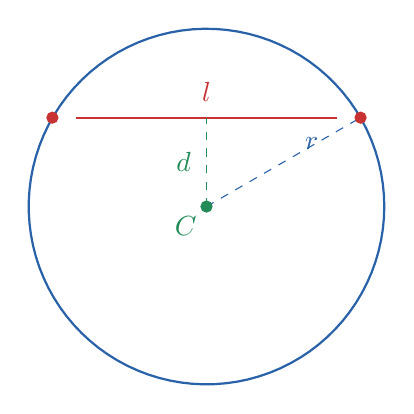
\begin{tikzpicture}
  \begin{axis}[
    width=7cm, height=7cm,
    axis lines=none,
    axis equal,
  ]
    \addplot[thick, mainblue, domain=0:360, samples=100] ({0+3*cos(x)},{0+3*sin(x)});
    % 弦
    \addplot[thick, warnred, domain=-2.2:2.2] {1.5};
    % 弦的端点
    \addplot[only marks, mark=*, mark size=2pt, warnred] coordinates {(-2.6, 1.5) (2.6, 1.5)};
    \node[warnred, anchor=south] at (axis cs:0,1.6) {$l$};
    % 圆心
    \addplot[only marks, mark=*, mark size=2pt, tipgreen] coordinates {(0, 0)};
    \node[tipgreen, anchor=north east] at (axis cs:0,0) {$C$};
    % 圆心到弦的距离
    \draw[dashed, tipgreen] (axis cs:0,0) -- (axis cs:0,1.5);
    \node[tipgreen, anchor=east] at (axis cs:-0.1,0.75) {$d$};
    % 半径
    \draw[dashed, mainblue] (axis cs:0,0) -- (axis cs:2.6,1.5);
    \node[mainblue, anchor=south west] at (axis cs:1.5,0.8) {$r$};
  \end{axis}
\end{tikzpicture}
\end{center}

% ============ 第二部分：例题精讲 ============
\section*{\textcolor{examorange}{二、例题精讲}}

\begin{examplebox}[【例题1】求直线的斜率和倾斜角]
已知直线 $l$ 经过点 $A(1, 2)$ 和 $B(3, 6)$，求直线 $l$ 的斜率和倾斜角。
\end{examplebox}

\textbf{解：}

由斜率公式得：
\[
k = \frac{y_2 - y_1}{x_2 - x_1} = \frac{6 - 2}{3 - 1} = \frac{4}{2} = 2
\]

由 $k = \tan\alpha = 2$，得倾斜角 $\alpha = \arctan 2$。

\begin{tipbox}[方法总结]
已知两点求斜率直接代公式；由斜率求倾斜角时，注意 $\alpha$ 的范围是 $[0°, 180°)$。当 $k > 0$ 时，$\alpha = \arctan k \in (0°, 90°)$。
\end{tipbox}

\bigskip

\begin{examplebox}[【例题2】求直线方程]
求过点 $(2, -1)$，且与直线 $3x - 2y + 4 = 0$ 平行的直线方程。
\end{examplebox}

\textbf{解：}

直线 $3x - 2y + 4 = 0$ 的斜率为 $k = \dfrac{3}{2}$。

因为所求直线与已知直线平行，所以所求直线斜率也为 $k = \dfrac{3}{2}$。

由点斜式得：
\[
y - (-1) = \frac{3}{2}(x - 2)
\]
化简为一般式：
\[
2(y + 1) = 3(x - 2) \implies 3x - 2y - 8 = 0
\]

\textbf{也可以用"设一般式"法：}设所求直线为 $3x - 2y + C = 0$，代入 $(2, -1)$：
$3 \times 2 - 2 \times (-1) + C = 0 \implies C = -8$。

故所求直线方程为 $\boxed{3x - 2y - 8 = 0}$。

\begin{tipbox}[方法总结]
与已知直线平行的直线可设为 $Ax + By + C = 0$（$A$、$B$ 不变，$C$ 待定），再代入已知点求 $C$。此法比用点斜式更简洁。
\end{tipbox}

\bigskip

\begin{examplebox}[【例题3】两直线的位置关系]
判断下列两直线的位置关系：
\begin{enumerate}[label=(\arabic*)]
  \item $l_1: 2x + 3y - 1 = 0$，$l_2: 4x + 6y + 5 = 0$
  \item $l_1: x - 2y + 3 = 0$，$l_2: 2x + y - 1 = 0$
\end{enumerate}
\end{examplebox}

\textbf{解：}

(1) 对比系数：$A_1 = 2, B_1 = 3, C_1 = -1$；$A_2 = 4, B_2 = 6, C_2 = 5$。

$A_1B_2 - A_2B_1 = 2 \times 6 - 4 \times 3 = 12 - 12 = 0$，所以两直线平行或重合。

再验证：$A_1C_2 - A_2C_1 = 2 \times 5 - 4 \times (-1) = 10 + 4 = 14 \neq 0$。

因此 $l_1 \parallel l_2$（\textbf{平行}）。

(2) $A_1 = 1, B_1 = -2$；$A_2 = 2, B_2 = 1$。

$A_1A_2 + B_1B_2 = 1 \times 2 + (-2) \times 1 = 2 - 2 = 0$。

因此 $l_1 \perp l_2$（\textbf{垂直}）。

\bigskip

\begin{examplebox}[【例题4】点到直线的距离]
求点 $P(3, -2)$ 到直线 $4x + 3y - 5 = 0$ 的距离。
\end{examplebox}

\textbf{解：}

由点到直线距离公式：
\[
d = \frac{|4 \times 3 + 3 \times (-2) - 5|}{\sqrt{4^2 + 3^2}} = \frac{|12 - 6 - 5|}{\sqrt{25}} = \frac{|1|}{5} = \boxed{\dfrac{1}{5}}
\]

\bigskip

\begin{examplebox}[【例题5】直线与圆的位置关系]
判断直线 $l: x - y + 1 = 0$ 与圆 $C: x^2 + y^2 - 4x - 2y + 1 = 0$ 的位置关系。
\end{examplebox}

\textbf{解：}

将圆的方程配方：$(x - 2)^2 + (y - 1)^2 = 4$。

圆心 $C(2, 1)$，半径 $r = 2$。

圆心到直线的距离：
\[
d = \frac{|2 - 1 + 1|}{\sqrt{1^2 + (-1)^2}} = \frac{2}{\sqrt{2}} = \sqrt{2}
\]

因为 $d = \sqrt{2} < 2 = r$，所以直线与圆\textbf{相交}。

\begin{center}
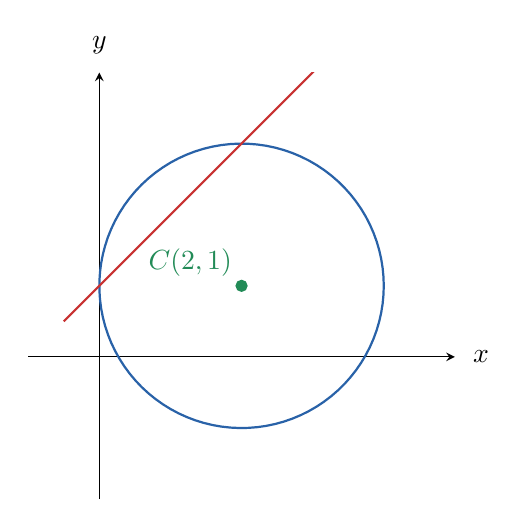
\begin{tikzpicture}
  \begin{axis}[
    width=7cm, height=7cm,
    axis lines=middle,
    xlabel={$x$}, ylabel={$y$},
    xmin=-1, xmax=5, ymin=-2, ymax=4,
    ticks=none, axis equal,
    every axis x label/.style={at={(ticklabel* cs:1.02)}, anchor=west},
    every axis y label/.style={at={(ticklabel* cs:1.02)}, anchor=south},
  ]
    \addplot[thick, mainblue, domain=0:360, samples=100] ({2+2*cos(x)},{1+2*sin(x)});
    \addplot[thick, warnred, domain=-0.5:4.5] {x+1};
    \addplot[only marks, mark=*, mark size=2pt, tipgreen] coordinates {(2, 1)};
    \node[tipgreen, anchor=south east] at (axis cs:2,1) {$C(2,1)$};
  \end{axis}
\end{tikzpicture}
\end{center}

\bigskip

\begin{examplebox}[【例题6】圆的切线方程]
求过点 $P(1, 3)$ 向圆 $x^2 + y^2 = 4$ 所作的切线方程。
\end{examplebox}

\textbf{解：}

圆心 $O(0, 0)$，半径 $r = 2$。

先验证点 $P$ 在圆外：$1^2 + 3^2 = 10 > 4$，点在圆外，故有两条切线。

\textbf{方法一：}设切线斜率为 $k$，切线方程为 $y - 3 = k(x - 1)$，即 $kx - y + 3 - k = 0$。

圆心到切线的距离等于半径：
\[
\frac{|k \cdot 0 - 0 + 3 - k|}{\sqrt{k^2 + 1}} = 2
\]
\[
\frac{|3 - k|}{\sqrt{k^2 + 1}} = 2 \implies (3 - k)^2 = 4(k^2 + 1)
\]
\[
9 - 6k + k^2 = 4k^2 + 4 \implies 3k^2 + 6k - 5 = 0
\]
\[
k = \frac{-6 \pm \sqrt{36 + 60}}{6} = \frac{-6 \pm \sqrt{96}}{6} = \frac{-6 \pm 4\sqrt{6}}{6} = \frac{-3 \pm 2\sqrt{6}}{3}
\]

故两条切线方程为：
\[
y - 3 = \frac{-3 + 2\sqrt{6}}{3}(x - 1) \quad \text{和} \quad y - 3 = \frac{-3 - 2\sqrt{6}}{3}(x - 1)
\]

\textbf{注意：}用斜率设方程时，不要遗漏斜率不存在的情况。本题中 $x = 1$ 不是切线（圆心到 $x = 1$ 的距离为 $1 < 2$），所以不需要补充。

\begin{tipbox}[方法总结]
求过圆外一点的切线方程，核心思路是利用"圆心到切线的距离 = 半径"。设斜率后列方程求解，注意检验斜率不存在的情况。
\end{tipbox}

\bigskip

\begin{examplebox}[【例题7】弦长计算]
直线 $y = x + 1$ 与圆 $x^2 + y^2 = 4$ 相交于 $A$、$B$ 两点，求弦 $AB$ 的长。
\end{examplebox}

\textbf{解：}

\textbf{方法一（几何法）：}

圆心 $O(0, 0)$ 到直线 $x - y + 1 = 0$ 的距离：
\[
d = \frac{|0 - 0 + 1|}{\sqrt{1^2 + (-1)^2}} = \frac{1}{\sqrt{2}} = \frac{\sqrt{2}}{2}
\]

半径 $r = 2$，故弦长：
\[
|AB| = 2\sqrt{r^2 - d^2} = 2\sqrt{4 - \frac{1}{2}} = 2\sqrt{\frac{7}{2}} = \sqrt{14}
\]

\textbf{方法二（韦达定理）：}

将 $y = x + 1$ 代入 $x^2 + y^2 = 4$：
\[
x^2 + (x + 1)^2 = 4 \implies 2x^2 + 2x - 3 = 0
\]

设两根为 $x_1, x_2$，则 $x_1 + x_2 = -1$，$x_1 x_2 = -\dfrac{3}{2}$。

\[
|x_1 - x_2| = \sqrt{(x_1 + x_2)^2 - 4x_1 x_2} = \sqrt{1 + 6} = \sqrt{7}
\]

弦长 $|AB| = \sqrt{1 + 1^2} \cdot |x_1 - x_2| = \sqrt{2} \cdot \sqrt{7} = \boxed{\sqrt{14}}$。

\begin{tipbox}[方法总结]
几何法利用勾股定理，代数法利用韦达定理。两种方法都应熟练掌握，几何法计算更简洁，代数法适用范围更广。
\end{tipbox}

\bigskip

\begin{examplebox}[【例题8】圆与圆的位置关系]
判断圆 $C_1: x^2 + y^2 = 4$ 与圆 $C_2: (x - 3)^2 + (y - 4)^2 = 9$ 的位置关系。
\end{examplebox}

\textbf{解：}

圆 $C_1$：圆心 $O_1(0, 0)$，半径 $r_1 = 2$。

圆 $C_2$：圆心 $O_2(3, 4)$，半径 $r_2 = 3$。

圆心距：$d = |O_1O_2| = \sqrt{3^2 + 4^2} = 5$。

因为 $r_1 + r_2 = 2 + 3 = 5 = d$，所以两圆\textbf{外切}。

\bigskip

\begin{examplebox}[【例题9】综合题——求圆的方程]
求以 $A(1, 3)$ 和 $B(5, 1)$ 为直径端点的圆的方程。
\end{examplebox}

\textbf{解：}

圆心为 $AB$ 的中点：$C = \left(\dfrac{1+5}{2}, \dfrac{3+1}{2}\right) = (3, 2)$。

半径为 $|AB|$ 的一半：
\[
|AB| = \sqrt{(5-1)^2 + (1-3)^2} = \sqrt{16 + 4} = 2\sqrt{5}
\]
\[
r = \frac{|AB|}{2} = \sqrt{5}
\]

圆的方程为：
\[
\boxed{(x - 3)^2 + (y - 2)^2 = 5}
\]

\bigskip

\begin{examplebox}[【例题10】对称问题]
求点 $A(2, 3)$ 关于直线 $l: x - y - 1 = 0$ 的对称点 $A'$ 的坐标。
\end{examplebox}

\textbf{解：}

设对称点 $A'(a, b)$。

\textbf{条件一：}$AA'$ 的中点在直线 $l$ 上。中点为 $\left(\dfrac{2+a}{2}, \dfrac{3+b}{2}\right)$，代入直线方程：
\[
\frac{2+a}{2} - \frac{3+b}{2} - 1 = 0 \implies a - b - 3 = 0 \quad \cdots (1)
\]

\textbf{条件二：}$AA' \perp l$。$AA'$ 的斜率为 $\dfrac{b - 3}{a - 2}$，直线 $l$ 的斜率为 $1$，故：
\[
\frac{b - 3}{a - 2} \times 1 = -1 \implies b - 3 = -(a - 2) \implies a + b - 5 = 0 \quad \cdots (2)
\]

联立 (1)(2)：
\begin{align*}
a - b &= 3 \\
a + b &= 5
\end{align*}
解得 $a = 4$，$b = 1$。

对称点为 $\boxed{A'(4, 1)}$。

\begin{tipbox}[方法总结]
求点关于直线的对称点，利用两个条件：(1) 中点在对称轴上；(2) 连线与对称轴垂直。联立方程组求解。
\end{tipbox}

% ============ 第三部分：应用题 ============
\section*{\textcolor{apppurple}{三、应用题}}

\begin{appbox}[【应用1】光线反射问题]
一束光线从点 $A(1, 2)$ 出发，经直线 $l: x + y = 0$ 反射后经过点 $B(3, 0)$，求反射光线的方程。
\end{appbox}

\textbf{解：}

利用光学反射原理，反射光线的延长线经过入射点关于镜面的对称点。

求 $A(1, 2)$ 关于直线 $x + y = 0$ 的对称点 $A'$。

设 $A'(a, b)$：
\begin{align*}
&\frac{1+a}{2} + \frac{2+b}{2} = 0 \implies a + b + 3 = 0 \quad \cdots (1)\\
&\frac{b-2}{a-1} \times (-1) = -1 \implies b - 2 = a - 1 \implies a - b - 1 = 0 \quad \cdots (2)
\end{align*}

联立得 $a = -1$，$b = -2$，即 $A'(-1, -2)$。

反射光线即为 $A'B$ 所在直线，斜率为 $k = \dfrac{0 - (-2)}{3 - (-1)} = \dfrac{1}{2}$。

反射光线方程：$y - 0 = \dfrac{1}{2}(x - 3)$，即 $\boxed{x - 2y - 3 = 0}$。

\bigskip

\begin{appbox}[【应用2】圆形花坛设计]
一个圆形花坛的圆心在点 $C(2, 3)$ 处，一条直线形小路的方程为 $4x + 3y - 25 = 0$。若要求花坛与小路相切，求花坛的半径。
\end{appbox}

\textbf{解：}

圆心 $C(2, 3)$ 到直线 $4x + 3y - 25 = 0$ 的距离为：
\[
d = \frac{|4 \times 2 + 3 \times 3 - 25|}{\sqrt{4^2 + 3^2}} = \frac{|8 + 9 - 25|}{5} = \frac{|-8|}{5} = \frac{8}{5}
\]

花坛与小路相切，半径等于圆心到小路的距离，故 $r = \boxed{\dfrac{8}{5}}$。

\bigskip

\begin{appbox}[【应用3】导航定位问题]
两座信号塔分别位于 $A(0, 0)$ 和 $B(6, 0)$ 处，信号覆盖范围均为 $4$ 千米。一辆汽车位于点 $P$，恰好同时被两座信号塔覆盖（即 $P$ 在两个信号覆盖圆的交集区域内）。求点 $P$ 到 $AB$ 中点的最大距离。
\end{appbox}

\textbf{解：}

两信号塔的信号覆盖范围分别为：
\[
\odot A: x^2 + y^2 \leqslant 16, \quad \odot B: (x - 6)^2 + y^2 \leqslant 16
\]

两圆交集区域的边界为两圆的交线。联立两圆方程：
\begin{align*}
x^2 + y^2 &= 16 \\
(x-6)^2 + y^2 &= 16
\end{align*}

相减得：$x^2 - (x-6)^2 = 0 \implies 12x - 36 = 0 \implies x = 3$。

代入 $x^2 + y^2 = 16$：$9 + y^2 = 16 \implies y^2 = 7 \implies y = \pm\sqrt{7}$。

$AB$ 中点为 $M(3, 0)$，点 $P$ 在 $x = 3$ 上时到 $M$ 的距离 $= |y| = \sqrt{7}$。

$P$ 同时在两圆内，$x = 3$ 时 $y$ 的范围为 $[-\sqrt{7}, \sqrt{7}]$。

因此点 $P$ 到 $AB$ 中点的最大距离为 $\boxed{\sqrt{7}}$ 千米。

% ============ 第四部分：课堂练习 ============
\section*{\textcolor{tipgreen}{四、课堂练习}}

\begin{enumerate}
  \item 已知直线 $l$ 的倾斜角为 $120°$，求直线 $l$ 的斜率。
  \item 求过点 $(1, -2)$，斜率为 $3$ 的直线方程。
  \item 已知直线 $l_1: 2x + y - 3 = 0$，$l_2: x - 2y + 1 = 0$，判断 $l_1$ 与 $l_2$ 的位置关系。
  \item 求平行线 $l_1: 3x - 4y + 5 = 0$ 与 $l_2: 3x - 4y - 7 = 0$ 之间的距离。
  \item 求以 $(1, -2)$ 为圆心，半径为 $3$ 的圆的标准方程。
  \item 判断直线 $y = 2x + 1$ 与圆 $x^2 + y^2 = 5$ 的位置关系。
  \item 求圆 $x^2 + y^2 - 6x + 4y - 12 = 0$ 的圆心和半径。
  \item 求点 $(2, -1)$ 到直线 $5x - 12y + 3 = 0$ 的距离。
\end{enumerate}

\bigskip

\begin{knowledgebox}[参考答案]
\begin{enumerate}
  \item $k = \tan 120° = \tan(180° - 60°) = -\tan 60° = -\sqrt{3}$。

  \item 点斜式：$y - (-2) = 3(x - 1)$，即 $3x - y - 5 = 0$。

  \item $A_1A_2 + B_1B_2 = 2 \times 1 + 1 \times (-2) = 0$，故 $l_1 \perp l_2$。

  \item $d = \dfrac{|5 - (-7)|}{\sqrt{9 + 16}} = \dfrac{12}{5}$。

  \item $(x - 1)^2 + (y + 2)^2 = 9$。

  \item 圆心 $(0, 0)$ 到直线 $2x - y + 1 = 0$ 的距离 $d = \dfrac{1}{\sqrt{5}}$。$r = \sqrt{5}$。$d = \dfrac{1}{\sqrt{5}} < \sqrt{5} = r$，直线与圆相交。

  \item 配方：$(x - 3)^2 + (y + 2)^2 = 25$。圆心 $(3, -2)$，半径 $r = 5$。

  \item $d = \dfrac{|5 \times 2 - 12 \times (-1) + 3|}{\sqrt{25 + 144}} = \dfrac{25}{13}$。
\end{enumerate}
\end{knowledgebox}

\vfill
\begin{center}
\small\textcolor{gray}{本讲义仅供教学参考，例题可根据学生水平调整难度。}
\end{center}

\end{document}
